\section{Experiments}
\subsection{Datasets}
The full benchmark study is designed for public HSI datasets including Indian Pines, Pavia University, Pavia Centre, Salinas, Houston 2013, and one WHU-Hi scene when available. These datasets cover agricultural, urban, and mixed land-cover environments and differ in spectral resolution, spatial size, number of classes, and annotation density. For each scene, unlabeled pixels are excluded from supervised metrics.

\subsection{Implementation Details}
The implementation is written in PyTorch. Each data cube is normalized band-wise, and PCA is optionally applied before patch extraction. Unless otherwise stated, the patch size is set to $9\times9$, the hidden dimension is 128, and AdamW is used for optimization. Each experiment is repeated over multiple random seeds. The best model is selected according to validation overall accuracy and evaluated once on the test split.

\subsection{Evaluation Metrics}
The main metrics are overall accuracy (OA), average accuracy (AA), Cohen's Kappa, Macro-F1, per-class accuracy, worst-class accuracy, rare-class accuracy, expected calibration error (ECE), and confusion matrix. OA measures the total proportion of correctly classified pixels. AA gives equal weight to each class and is therefore more informative under imbalance. Macro-F1, worst-class accuracy, and rare-class accuracy directly evaluate the reliability-oriented claim. Kappa evaluates agreement beyond chance. Mean uncertainty, ECE, and uncertainty maps are also reported to analyze ambiguous predictions.

\subsection{Baselines}
Recommended baselines include 3D-CNN, HybridSN, SSRN, SpectralFormer or SSFTT, a graph-based classifier, a recent Mamba-based classifier, and SCATNet when comparing against the authors' previous work. The final submission should use official code when available or carefully reimplemented baselines under the same splits.

\subsection{Ablation Study}
The ablation study removes the spectral state-space branch, graph branch, robust loss, prototype head, and graph smoothness term independently. Additional experiments should vary the number of labeled samples per class and introduce controlled label noise. This design tests whether each component improves not only accuracy but also stability.

\subsection{Pipeline Verification}
Before full benchmark training, a synthetic HSI scene was used to verify the code path. The smoke test confirms that data loading, PCA, patch extraction, model training, validation, testing, checkpoint saving, metric logging, table generation, and figure generation execute end-to-end. These synthetic results are not intended as scientific evidence; they are included only to verify reproducibility infrastructure.

\begin{table}[t]
\centering
\caption{Pipeline verification results generated from a short synthetic run. These values are not final benchmark results.}
\begin{tabular}{lc}
\hline
Metric & DR-GSMamba \\
\hline
OA & 60.07 $\pm$ 0.00 \\
AA & 60.09 $\pm$ 0.00 \\
Kappa & 54.41 $\pm$ 0.00 \\
Macro-F1 & 59.41 $\pm$ 0.00 \\
Worst-Class Acc. & 47.35 $\pm$ 0.00 \\
Rare-Class Acc. & 59.67 $\pm$ 0.00 \\
ECE & 5.61 $\pm$ 0.00 \\
\hline
\end{tabular}

\label{tab:pipeline}
\end{table}

\begin{figure}[t]
\centering
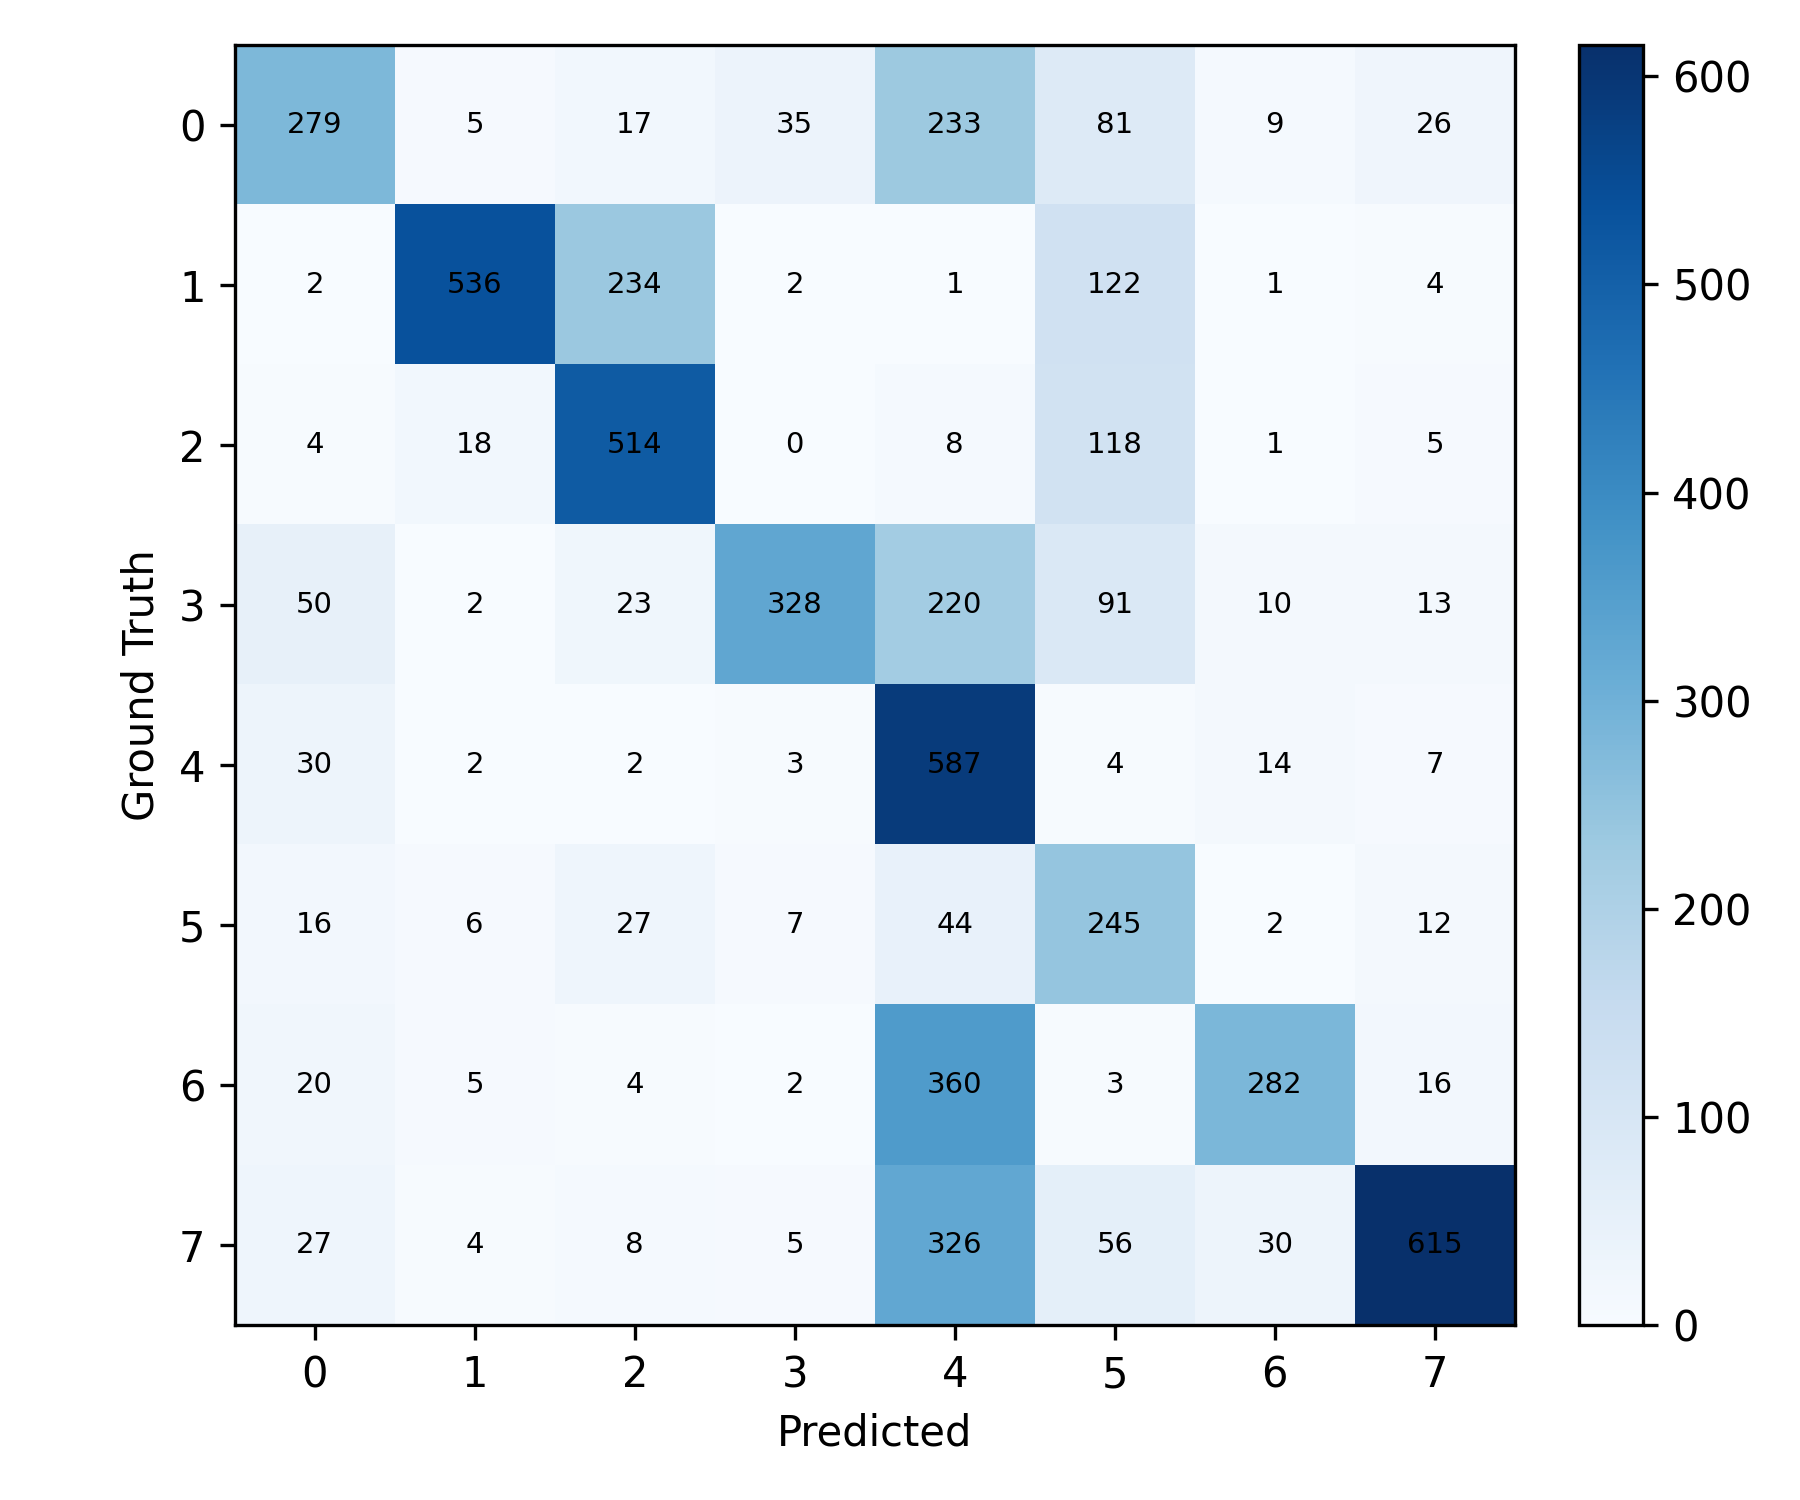
\includegraphics[width=0.9\linewidth]{figures/confusion_matrix.png}
\caption{Confusion matrix generated from the synthetic smoke-test split. This figure verifies the automatic paper asset pipeline.}
\label{fig:cm}
\end{figure}

\subsection{Expected Final Reporting}
For a journal submission, Table~\ref{tab:pipeline} must be replaced by benchmark results on real datasets. The final paper should include a main comparison table, per-class accuracy tables, ablation tables, classification maps, uncertainty maps, stability boxplots over random seeds, and a computational cost comparison. The repository already stores all metrics in JSON format, making these assets reproducible from experiment outputs.
